\documentclass[conference]{IEEEtran}
\IEEEoverridecommandlockouts
% The preceding line is only needed to identify funding in the first footnote. If that is unneeded, please comment it out.
\usepackage{cite}
\usepackage{amsmath,amssymb,amsfonts}
\usepackage{algorithmic}
\usepackage{graphicx}
\usepackage{textcomp}
\usepackage{xcolor}
\usepackage{CJKutf8}
\def\BibTeX{{\rm B\kern-.05em{\sc i\kern-.025em b}\kern-.08em
    T\kern-.1667em\lower.7ex\hbox{E}\kern-.125emX}}
\begin{document}
\begin{CJK*}{UTF8}{gbsn}
\title{The paradox of Machine Translation base on Sentiment Analysis polarity:
  using Metamorphic Testing}

\author{\IEEEauthorblockN{1\textsuperscript{st} Boyang Yan}
\IEEEauthorblockA{\textit{Research Center of Network and Communications} \\
\textit{Peng Cheng Laboratory}\\
Shenzhen, China \\
yanby@pcl.ac.cn}
\and
\IEEEauthorblockN{2\textsuperscript{nd} Given Name Surname}
\IEEEauthorblockA{\textit{dept. name of organization (of Aff.)} \\
\textit{name of organization (of Aff.)}\\
City, Country \\
email address}
\and
\IEEEauthorblockN{3\textsuperscript{rd} Given Name Surname}
\IEEEauthorblockA{\textit{dept. name of organization (of Aff.)} \\
\textit{name of organization (of Aff.)}\\
City, Country \\
email address}
\and
\IEEEauthorblockN{4\textsuperscript{th} Given Name Surname}
\IEEEauthorblockA{\textit{dept. name of organization (of Aff.)} \\
\textit{name of organization (of Aff.)}\\
City, Country \\
email address}
\and
\IEEEauthorblockN{5\textsuperscript{th} Given Name Surname}
\IEEEauthorblockA{\textit{dept. name of organization (of Aff.)} \\
\textit{name of organization (of Aff.)}\\
City, Country \\
email address}
\and
\IEEEauthorblockN{6\textsuperscript{th} Given Name Surname}
\IEEEauthorblockA{\textit{dept. name of organization (of Aff.)} \\
\textit{name of organization (of Aff.)}\\
City, Country \\
email address}
}

\maketitle

\begin{abstract}
A huge amount of text comments are posted on different topics in Social Media
 every day. These topics are discussed in different languages by
 different language speakers. It is necessary for people to use machine
 translation tools in global integration. However, accuracy and reliable of
 machine translation tools services is paying close attention by users. The
 quantity of machine translation services and difficult translation text
 evaluation have been a hot area of research for several years. It is important
 for improving the quality of machine translation services to narrow the
 research gap. The purpose of the paper is to explore what kind of text is
 difficult to translate for machine translation services base on movie comments
 data in Douban Movie Community Website. Metamorphic Testing is main method for
 establishing a testing model which using Google Sentiment Analysis tool to
 analyze original Chinese movie comments dataset and English translated
 datasets, which are Google Translation dataset, Yandex Translation dataset and
 Baibu Translation dataset, both side (Chinese and English) should be same
 emotional polarization (positive or negative). If the results are opposite
 polarization, that means this sentence is difficult for machine translation. As
 a result, people will able to use this testing model finding difficult
 sentences and doing specific optimiztion. The research result shows that the
 three translation tools overall quality are poor based on Receiver operating
 characteristic(ROC) curve and precision-recall curve (PRC).
 In addition, there are outstanding language problems in machine translation,
 computer science researchers must be combined with linguistic researchers, so
 further research of Machine translation should pay enough attention to
 linguistics research, the expansion of corpus, vocabulary differentiation,
 grammatical analysis and so on, should be deeply and comprehensively studied.

\end{abstract}

\begin{IEEEkeywords}
  Metamorphic Testing, machine translation, MT4MT, sentiment analysis, machine
  translation quantity testing, evaluation of machine translation services
  difficult, natural language, Receiver operating characteristic(ROC) curve,
  precision-recall curve (PRC)
\end{IEEEkeywords}

\section{Introduction}
Most people encounter language and cultural barriers during cross-language
communication. There are lots of text and documents on different languages need
to translation every day. It would be impossible to translation the huge amount
of data generated manually. Nowadays, there are lots of machine translation
tools are available in the world, such as Google translation, Bing translation,
Yandex, Baidu translation and Youdao translation and so on. Machine translation
services has been becoming more and more widely used, also more and more
popular. It is necessary for global integration to use Cross-language machine
translation tools. In especial, machine translation system has significantly
increased international trade \cite{brynjolfsson2018does}. Most research only
focuses on ranking the quantity of machine translation services in some field
\cite{pesu2018monte, aiken2010efficacy, koehn2006manual, somers2005round,
  shigenobu2007evaluation} but little research has conducted on difficult
translation text evaluation. In this paper, all of testing data (Origin Chinese
dataset) from DOUBAN, which is an Social Media website about books, movies,
music, to study the translation quality of different translation tools.
Douban film is China's largest and most authoritative
film sharing and comment community \cite{Douban}.
Social Media has been becoming more and more widely used.
Accounting to Perrin’s survey, there are only $7%$ American adults are use
social media in 2005. However, social media usage increase rapidly, there are
$65%$ American adults are use social media until 2015 \cite{perrin2015social}.
Social Media website comment text from the language word level has its unique
style, such as the text has colloquial vocabulary for the convenience of
expression. At present, it is urgent to carry out in-depth study
on this field, which may open up the new field of theoretical research.
In this study, we only fouced on three of Machine Translation tools, which are
Google, Yandex and Baidu.
Google translation tool come from American, Yandex come from Russia, and Baidu
come from China. This three tools all come from the top three powerful country.
Accounting to Pesu said machine translation tools can product better results on
European languages compare with Asian language \cite{pesu2018monte}. So, form
Chinese to English translation tool is the main kind of translation languages to
analysis translation difficults in the paper. Evaluation of machine translation
services difficults usually need language expert, who need well-known both languages, to
participate. However, language expert also involves human emotional judgment.
Automatic assessment human language is naturally difficult because of without a
test oracle \cite{zhou2016metamorphic}. In this paper, achieving a testing modle to automatic
assessment without language expert. Metamorphic testing(MT) is one of
property-based software quality testing method, which alreadly be appoved
effective for addressing the oracle problem, such as testing the quality of
search engine and the quality of Unmanned Aerial Vehicle(UAV) flight control
application and so on. Therefore, decideing metamorphic testing to find machine
translation services difficults in non-oracle sitation. And more specifically,
this research raise two questions.

\begin{itemize}
  \item Q1: What is current sitation of the quantity of Chinese to English
    machine translation?
  \item Q2: What is current machine translation difficults between Chinese and English?
\end{itemize}

The rest of paper is organized as three parts. Firstly, domonstration the
quantity of Chinese to English translation services. This part addresses Q1.
secondly, describtion testing model about finding the difficults of machine
translation. Thirdly, analyzes the experimental results and discussion. This part will
answer Q2.

\section{Background}
\subsection{Metamorphic Testing}
Metamorphosis Testing (MT) is a method for generating test cases, as well as test
results verification \cite{zhou2017introduction}. The most importance component is the metamorphic
relation (MR) \cite{chen2003fault}. MR is the target application's necessary
properties of function in relation to multiple inputs and their expected outputs.
MT has been researched through more and more researchers constantly strive
toward and adopted by industries and organizations such as Adobe, NASA and the
National Institute of Standards and Technology \cite{zhou2018metamorphic}.
In software testing research field, an incapacity to decide, software product
the correct output, is called the oracle problem \cite{brown2018metamorphic}.
This usually means cannot provide exact correctness reference data. such as,
machine translation. Huge and complexity systems, does not have
reference data for proving function's correctness, is very common.
When people want to assess the the accuracy of $\sin$ function. For example, $\sin(2.7)$ is very difficult to
make a correctness judgment from mathematics aspect. If using Metamorphic
Testing method to testing $\sin$ function will reduce computational costs and
more efficient. There is a testing procedures' example for $\sin$ function.
\begin{enumerate}\label{itm:procedures}
\item set a Metamorphic Relation: such as $$\sin(\alpha) = \cos(\frac{\pi}{2} - \alpha)$$
\item $\sin(2.7)$ and $\cos(\frac{\pi}{2} - 2.7)$ should have same output, if the
  outputs are different. We can say, this MR have been break, maybe the failure
  have been detected.
\end{enumerate}
However, when using \ref{itm:procedures}'s testing procedures. Someone maybe
ask, $\cos$ function also not reliable, how can use a unreliable function to
test another function's correctness. There have the boundedness. However, both
function have got failures at same time, that is small probability event.
\subsection{Sentiment Analysis}
Sentiment analysis is a part of text data mining. The aim of sentiment analysis
is to determine the attitude of speakers or writers with respect to particular
topics or the overall contextual polarity or emotional reaction to a text
document. It is usually equated with opinion mining, which involves the use of
natural language processing and machine learning to ascertain the possibility of
positive or negative opinions \cite{yadollahi2017current}. Sentiment analysis is useful for analyzing a
huge amount of data relating to personal opinions. It can be used in an
e-business context. For example, business managers can analysis customers’
attitudes, as to whether they like or dislike their product or service. Also,
government can use sentiment analysis to analyze citizen perspectives.
In this paper, we will using Google Sentiment Analysis tool to prove the the
quantity of Machine Translation. The details of Testing Modle will talk in \ref{testingModle} .

\section{domonstration the current quantity of Chinese to English translation
  services} \label{currentQuantity}

\subsection{Test Sample}
All of test sample came from Douban\footnote{Douban Website:
  https://www.douban.com/}, one of biggest social networking service
platforms in China. This social website attracts more than one hundred million
active visitors per month, and has amassed over sixty-five million registered
users \cite{doubanStat}. We then employ the Douban public Application Programming Interfaces
(APIs) to access Chinses-written comments. A typical data structure of harvested
comment is shown as a tuple: [Rating, Raw comments]. Totally, comments have got
46180 in the corpus. User rating total have 5 groups, which are 10, 20, 30, 40
and 50, from negative to positive.
The test sample distribution diagram on below.
\begin{figure}[h]
  \centering
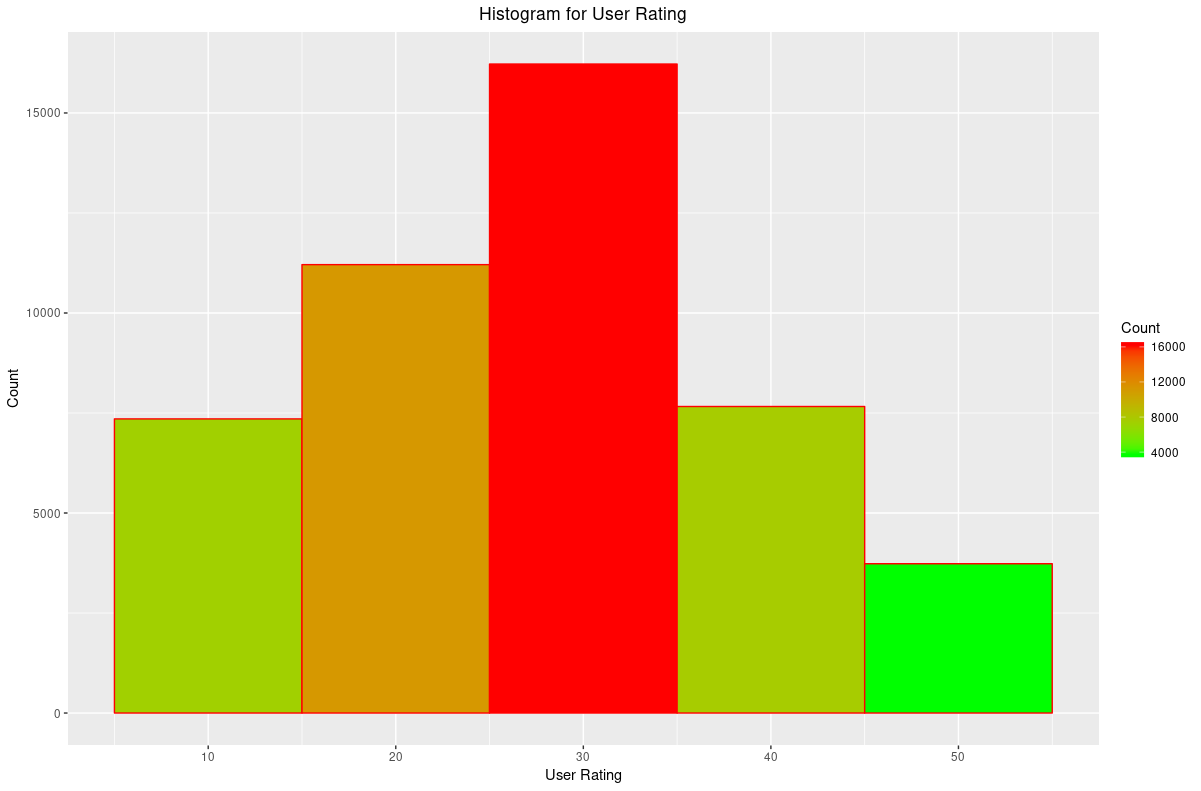
\includegraphics[width=0.3\paperwidth]{./img/ratingHis.png}
\caption{User Rating Histogram}
\label{fig:userRatingHistogram}
\end{figure}
As you can see, the majority of comments allocate on rating 30. In addition,
there have got more negative comments compare with positive comments.

\subsection{Testing procedures} \label{testingModle}
\begin{figure}[h]
  \centering
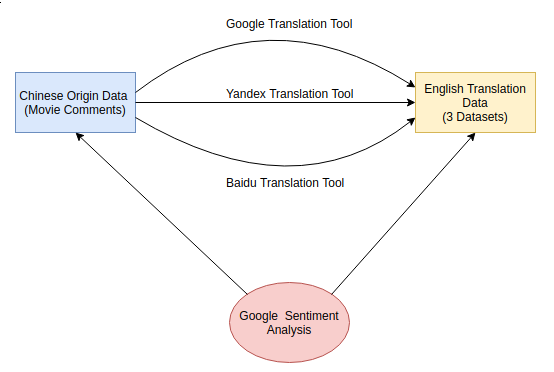
\includegraphics[width=0.35\paperwidth]{./img/model.png}
\caption{Testing Procedures}
\label{fig:testingProcedures}
\end{figure}
One the below, will explain more details for figure \ref{fig:testingProcedures}.

\begin{enumerate}
  \item using three of machine translation services to translate Chinese
    original movie comments to English translated movie comments.
    $$P_{(Origin Data)} \rightarrow P^{\prime}_{(Google Translation)}$$
    $$P_{(Origin Data)} \rightarrow P^{\prime}_{(Yandex Translation)}$$
    $$P_{(Origin Data)} \rightarrow P^{\prime}_{(Baidu Translation)}$$
  \item Using Google sentiment analysis tool to analysis $P_{(Origin Data)}$,
    $P^{\prime}_{(Google Translation)}$, $ P^{\prime}_{(Yandex Translation)}$ and $
    P^{\prime}_{(Baidu Translation)}$. Google sentiment analysis APIs will get 2
    values, which are Score and Manitude. The range of Score is between -1 and
    1. If Score more close to 1 means this movie comment more positive, as well
    as, if Score more close to -1 means this movie comment more negative. In
    this paper, we have not analysis Manitude, which for distinction mix and neutral.
  \item\label{itm:testingProcedure3} Using user rating values (10, 20, 30, 40 or 50) to check Google
    Sentiment Analysis(SA) results $P_{(Origin Data)} $ is True or False. For
    example, user rating = 10 and Google Chinese SA score between -1
    and -0.6 (mean True) user ranking = 10 and Google Chinese SA score bigger
    than -0.6 (mean False). The decideing True table on below.\\
     \begin{table}[h]
      \caption {The Range of Score: True/ False}
     \begin{center}
      \begin{tabular}{|c|c|c|c|}
        \hline
        user rating & Google SA score & True/False \\
        \hline\hline
        10 & $[ \, -1, -0.4 ] \,$ & True \\
        \hline
        20 & $[ \, -0.8, 0 ] \,$ & True \\
        \hline
        30 & $[ \, -0.4, 0.4 ] \,$ & True \\
        \hline
        40 & $[ \, 0, 0.8 ] \,$ & True \\
        \hline
        50 & $[ \, 0.4, 1 ] \,$ & True \\
        \hline \hline
        10 & $( \, -0.4, 1 ] \,$ & False \\
        \hline
        20 & $[ \, -1, -0.8) \,$ & False \\
        \hline
        20 & $( \, -0.8, 1] \,$ & False \\
        \hline
        30 & $[ \, -1, -0.4) \,$ & False \\
        \hline
        30 & $( \, 0.4, 1] \,$ & False \\
        \hline
        40 & $[ \, -1, 0) \,$ & False \\
        \hline
        40 & $( \, 0.8, 1] \,$ & False \\
        \hline
        50 & $[ \, -1, 0.4) \,$ & False \\
        \hline
        \hline
      \end{tabular}
    \end{center}
  \end{table}

    As you can see, the Google SA score ranges have got some overlap because
    overlap can decrease the results, machine translation evaluation
    correctness, influence by the accuracy of Google Sentiment Analysis tool.
  \item Using those True or False values as vector combining with Google English
    SA scores (based on $P^{\prime}_{(Google Translation)}$), Google English SA
    scores (based on $ P^{\prime}_{(Yandex Translation)}$) and Google English SA
    scores (based on $P^{\prime}_{(Baidu Translation)}$) draw 3 Receiver operating
    characteristic (ROC) graphics and 3 Precision-recall curves (PRC) graphics.

    ROC curve is often used in evaluation the clinical performance of a
    biochemical test \cite{zweig1993receiver}. The ROC curve is based on a
    series of different binary
    classifier with the true positive rate (sensitivity) as the Y-axis and the
    false positive rate (1-specificity) as the X-axis \cite{ROC}. The traditional
    evaluation must be divided into two categories, and then statistical
    analysis is performed. The ROC curve is different from the traditional
    evaluation method. Instead, an intermediate state is allowed. The test
    results can be divided into multiple ordered classifications then
    statistically analyzed. However, visual interpretation and comparisons of
    ROC curves based on imbalanced data sets can be misleading. An alternative
    to a ROC curve is a precision-recall curve (PRC). PRC might be a better
    choice for imbalanced datasets \cite{davis2006relationship}.
    This graphic show those three of machine translation tools all achieve poor
    translation results.
\begin{figure}[h]
  \centering
    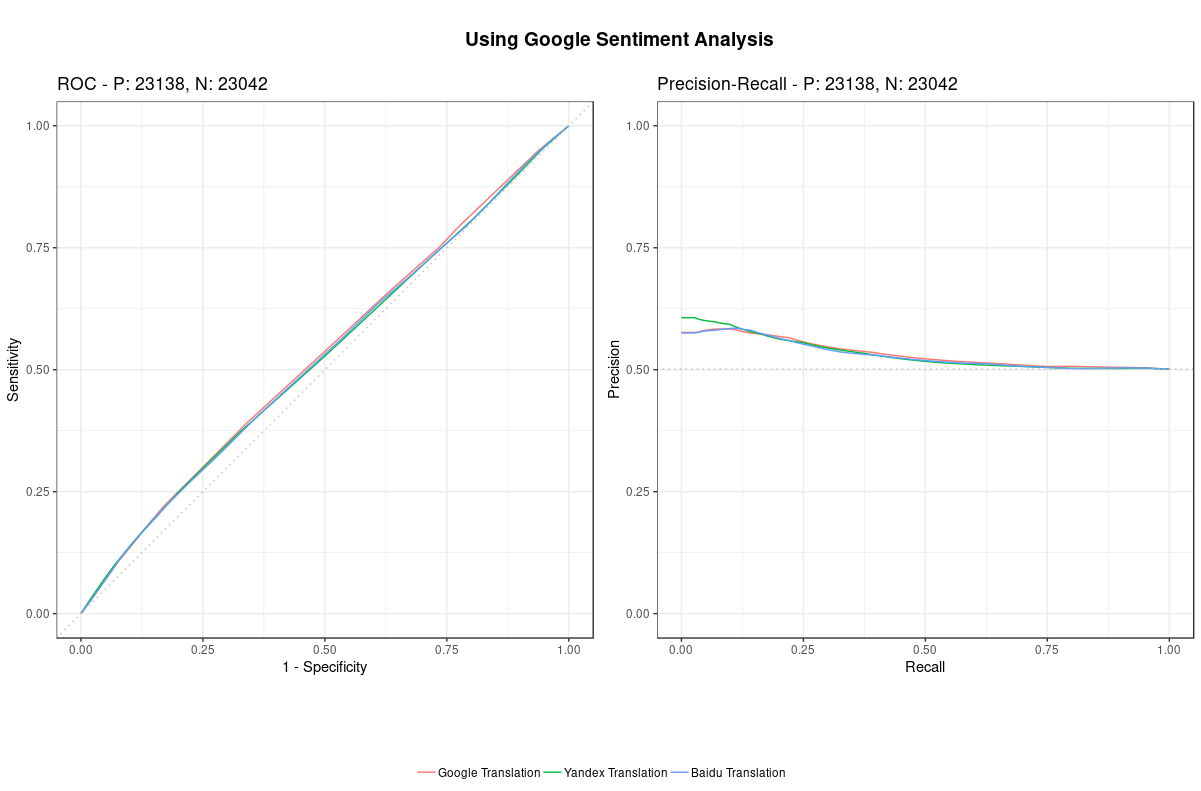
\includegraphics[width=0.35\paperwidth]{./img/ROCandPRC.png}
\caption{ROC and PRC graphics}
\label{fig:ROCandPRC}
\end{figure}
  \item Calculate Area Under The Curve (AUC) values for ROC and PRC.
    \begin{table}[h]
      \caption {Google Translation}
    \begin{center}
      \begin{tabular}{|c|c|}
        \hline
        Curve Types & AUCs \\
        \hline\hline
        ROC & 0.5307797 \\
        \hline
        PRC & 0.5328503 \\
        \hline
      \end{tabular}
    \end{center}
  \end{table}
   \begin{table}[h]
     \caption {Yandex Translation}
     \begin{center}
       \begin{tabular}{|c|c|}
         \hline
         Curve Types & AUCs \\
         \hline\hline
         ROC & 0.5251734 \\
         \hline
         PRC & 0.5322736 \\
         \hline
       \end{tabular}
     \end{center}
   \end{table}
  \begin{table}[h]
    \caption {Baidu Translation}
    \begin{center}
      \begin{tabular}{|c|c|}
        \hline
        Curve Types & AUCs \\
        \hline\hline
        ROC & 0.5258386 \\
        \hline
        PRC & 0.5302736 \\
        \hline
      \end{tabular}
    \end{center}
  \end{table}\\
  The AUC is between 1.0 and 0.5. The better diagnostic effect will be close to
  1. The ranking of accuracy is show on Table: \ref{accuracyJudgment}\\\\
  \begin{table}[h]\label{accuracyJudgment}
    \caption {ROC and PRC accuracy judgment}
     \begin{center}
       \begin{tabular}{|c|c|}
         \hline
         AUC value & Accuracy \\
         \hline\hline
         $[ \, 0.5, 0.7] \,$ & lower accuracy \\
         \hline
         $[ \, 0.7, 0.9] \,$ & certain accuracy \\
         \hline
         $[ \, 0.9, 1] \,$ & higher accuracy \\
         \hline
       \end{tabular}
     \end{center}
   \end{table}
  When AUC=0.5, it means that the diagnostic method is completely ineffective
  and has no diagnostic value \cite{baiduROC}.
\end{enumerate}
  \subsection{Current Translation Tool Results Analysis}
  In the testing Procedures \ref{itm:testingProcedure3}, which is the judgment of Google Chinese
    Sentiment Analysis(SA) results is True or False, there are totally have find
    23042 of true value, as well as 23138 of false value. Alought the dataset is
    looks balanced, ROC diagram can be trusted. The ranking of machine
    translation services' quantity are NOT reliable. The reason is three of
    translation services have lower accuracy. In another word, working not
    properly correct. However, there are still have the ranking of machine
    translation services' quantity on the below.
\subsubsection{For ROC AUCS}
\textbf{It shows Google Translation tool better than Baidu Translation tool better than Yandex Translation tool}
\subsubsection{For PRC AUCS}
\textbf{It shows Googl Translation tool better than Yandex Translation tool better than Baidu Translation tool}

\section{finding the difficults of machine translation}
\subsection{Testing procedures}
The first two step is same with, showing the current quantity of Machine
Translation Tools in Section \ref{currentQuantity}. Which are get translated
datasets and sentiment analysis for 4 datasets(Chinese Origin dataset, Yandex
translation dataset, Google translation dataset and Baidu translation dataset).
The only different is filting all of opposite polarization (very positive or
very negative) datasets and create three of Metamorphic Relation (MR).
\subsubsection{MR1}
$$SA_{(Origin Data)} \approx SA^{\prime}_{(Google Translation)}$$
\subsubsection{MR2}
$$SA_{(Origin Data)} \approx SA^{\prime}_{(Yandex Translation)}$$
\subsubsection{MR3}
$$SA_{(Origin Data)} \approx SA^{\prime}_{(Baidu Translation)}$$
\subsection{Analysis}
MR1, MR2 and MR3 have got failures decideing by one side greater than 0.7 and
another side smaller than -0.7. In this paper, using veen diagram for show
failures distribution.
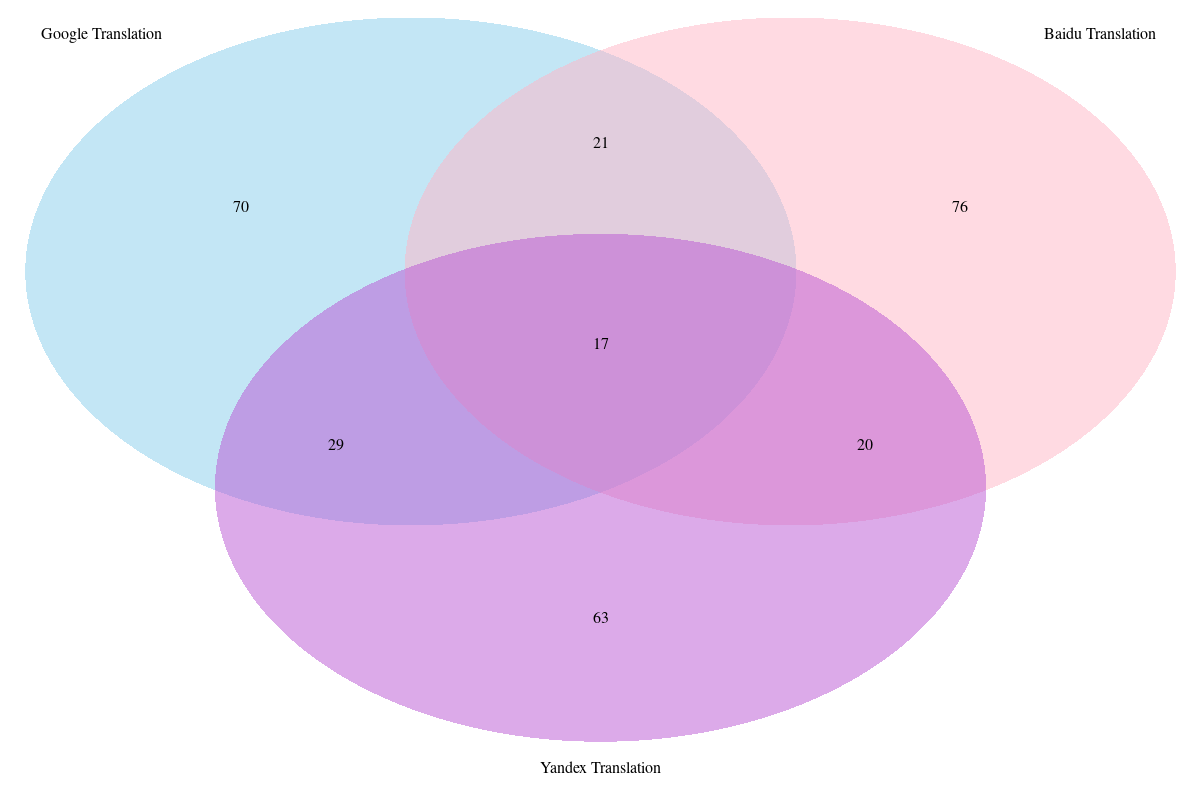
\includegraphics[width=0.35\paperwidth]{./img/veen.png}
  \begin{table}[h]
    \caption {Translation Failures Distribution}
    \begin{center}
      \begin{tabular}{|c|c|}
        \hline
        Types & Number Of Failures \\
        \hline\hline
        google Translation & 137\\
        \hline
        Yandex & 129 \\
        \hline
        Baidu & 134 \\
        \hline
        $Google \cap Baidu$ & 38 \\
        \hline
        $Google \cap Yandex$ & 46 \\
        \hline
        $Yandex \cap Baidu$ & 37 \\
        \hline
        $Yandex \cap Baidu \cap Google$ & 17 \\
        \hline
      \end{tabular}
    \end{center}
  \end{table}\\\\

\section{Language Analysis}
Google Translation, Yandex Translation and Baibu Translation are created by
different countries for different audiences, that is to say, the users of groups
are different. But Google Translation, Yandex Translation and Baidu Translation
exist lexical and grammatical problems, and some mistranslation is almost
coincide. The following aspects are the main common problems.
\subsection{Vocabulary Errors}
 The points of mistake are mainly manifested as the abuse of vocabulary,
 incorrect usage, the chaotic sequence, missing vocabulary,as well as improper
 selection of words.\\
 Examples:
 \subsubsection{fragmention sentence}
\begin{itemize}
\item Chinese \underline{Origin Movie comment} is:
  \begin{center}
    ``2013最后一场电影 就为恶心画一句号吧''
  \end{center}
\item The \underline{correct of the translation} is:\\
    ``This is the last movie in 2013. Let's make a full stop for all of nauseating  movie''
\item The \underline{Google Translation} is:
  \begin{center}
    ``Let's take a look at the last movie of 2013''
  \end{center}
\end{itemize}
  This is extremely negative comment. The hidded meaning is, this is nauseating
  movie. The Google translated sentence is fragmented and incomplete only
  translated the first part of original sentence.

 \subsubsection{misunderstand of vocabulary}
\begin{itemize}
\item Chinese \underline{Origin Movie comment} is:
  \begin{center}
    ``这片子真垃圾 就最后一点看起来比较有新意''
  \end{center}
\item The \underline{correct of the translation} is:\\
  ``This is really crap movie. However, the last part of movie is considerable innovative.
\item The \underline{Google Translation} is:\\
  ``This piece of real garbage on the last point looks more innovative''
\item The \underline{Yandex Translation} is:\\
  ``This film is really garbage it finally looks relatively new''
\item The \underline{Baidu Translation} is:\\
  ``The film is really garbage and it looks new at the last point.''
\end{itemize}
The original Chinese sentence front part is negative, but the back half sentence
is positive. This three of machine translation tools have got lots of vocabulary
misunderstand. such as, $$ movie \rightarrow piece $$ $$last\ part\ of\ movie \rightarrow finally\
or\ the\ last\ point$$

Besides,
\begin{itemize}
\item Chinese \underline{Origin Movie comment} is:
  \begin{center}
    ``剧本不好,梗比较生硬,有点无厘头。''
  \end{center}
\item The \underline{correct of the translation} is:\\
  ``The scenario is not good, the punchline of movie is stiff and a little bit
  does not make sense.''
\item The \underline{Google Translation} is:\\
  ``The script is not good, terrier stiffer, a bit nonsense.''
\item The \underline{Yandex Translation} is:\\
  ``The script is bad, stem relatively stiff, a bit does not make sense.''
\item The \underline{Baidu Translation} is:\\
  ``The script is not good, the stem is relatively stiff, a little silly.''
\end{itemize}
The original Chinese sentence is clear negative. All of three tools have got
problem with punchline of movie, ``梗'' is the internet lingo word. All of tools
need to improve the Internet lingo words. In addition, three of translation
tools also have got others misinterpretation of professional terms and literary
terms. such as ``春晚'' (Spring Festival Gala Show).

\subsection{Grammatical Errors}
The machine translation have got lots of grammatical mistake, such as sequence
disorder, improper location of adverbial attributive. The subject, the
predicate, the attributive, the adverbial, and the object is incomplete, etc.
\subsubsection{Illogical connect}
\begin{itemize}
\item Chinese \underline{Origin Movie comment} is:
  \begin{center}
    ``明明是搞笑片最后弄成了教育片''
  \end{center}
\item The \underline{correct of the translation} is:\\
  ``Obviously it is a comedy,but it made into educational films finally''
\item The \underline{Baidu Translation} is:\\
  ``It's a funny movie that finally makes an education film''
\end{itemize}
The ``that'' is illogical to connect Subject part and subordinate clause.
\subsubsection{Incomplete ingredients}
Origin Chinese sentence is ``中间确实无聊得很,但是结尾不赖''. The original
sentence meaning ``It's really boring in the middle part, but it's not bad at
the end''. The Yandex Translation ``The middle of really boring very, however at the end''.
\subsubsection{Sequence Disorder}
``想过是烂片,只是没想到能烂到这种地步,太应付了,一个星期拍完的吧''
Google
``Think of a bad movie, but did not expect to be able to rot to this point, too
coping, a week finished it''
Yandex
``Thought is a bad film, just didn't think it could be rotten to the point where
too cope with, a week finished.''
baidu
``That is a bad film, but did not expect to come to this rotten, too for a week, finished.''


The problem of sentence structure.Incomplete sentence composition, confusion of
words order.

For example, original sentence meaning”A few small cups of grape
juice, it is not very fresh”.GoogleTranslation ”A few small cups of grape juice,
very fresh”in completely different meaning;


Take another example,original
sentence meaning “ The first story is good, but the other is too
contrived”.
YandexTranslation”On the first story good the other is too
contrived”;


Besides,For example,original sentence meaning “The first half was
good with heavy irony, but the last apology was a little
redundant”.

BaiduTranslation”The first half was good - the irony was very heavy,
and the last apology was a little redundant”. Improper location of clauses”-”.
The misuse of conjunctions”and”.

The problem of sentence structure.Causality is unclear. For example,original
sentence meaning "I can not ignorant conscience to give too few stars,because I
am a gentle person”.GoogleTranslation "I am a gentle person, and I really do not
have the heart to give too few stars. . .”

Take another example,original sentence meaning “Bad,I will never see Feng
Xiaogang's movie again.”  YandexTranslation “Sucks, feel Feng Xiaogang movie
later never to see.”


从以上以豆瓣电影评论为分析对象来讨论这三个翻译软件的译文共同的问题,从整体上看,
无论是用词还是语法都一定的错误导致许多译文意思不准确,内容残缺,结构错误。

 From the overall points of view, above the Douban film review as the analysis
 object to discuss GoogleTranslation, YandexTranslation and BaiduTranslation
 tools common problems, whether the usage of words or grammar are a certain
 error caused by many translation inaccurate meaning, incomplete content, and
 the wrong structure.

 The reasons are colloquial language characters of Douban film review text and
 insufficient machine vocabulary.Although the length of the movie commentary
 sentences is short, the vocabulary is not difficult and the sentences’structure
 seems simple, there have got lots of colloquial speech and many of words are
 not formal, which is the main reason for the low quality of translation
 results. Lots of compound sentence is hidded. It is more difficult for
 intelligent machines translation services.Although the length of the movie
 commentary sentences is short, the vocabulary is not difficult and the
 sentences’structure seems simple, there have got lots of colloquial speech and
 many of words are not formal, which is the main reason for the low quality of
 translation results. Lots of compound sentence is hidded. It is more difficult
 for intelligent machines translation services.

 Although the length of the movie commentary sentences is short, the vocabulary
is not difficult and the sentences' structure seems simple, there have got
lots of colloquial speech and many of words are not formal, which is the main
reason for the low quality of translation results. Lots of compound
sentence is hidded. It is more difficult for intelligent machines translation
services.

Although the online translation text comments and review is short in length, but
more colloquial is serious, the use of words is not standard, so vocabulary
translation is more difficult.Although the sentence structure seems simple, but
hides the compound sentence, but the sentence pattern is rich and
complex.Besides,Differences in thinking between Chinese and English is more
difficult for intelligent machines, which is the main difficulty in the quality
difficulties of translation

 \section{Conclusion and Limitations}
In general, Google Translation, Yandex Translation and Baidu Translation tools
can still translate the basic meaning of a sentence. They are basically fluent
and understandable. However, all of three Machine Translation tools are poor
quality and similar. As you can seen, this tesing model is possible to detected Machine
Translation failures without language expert. But, there have got limitation in
the accuracy of Sentment Analysis tool, which difficult to distinguish minimal
change of emotion. As a results, this testing model will missing most of Machine
Translation failures, particularly, neutral emotional sentences. This tesing
model is good for decideing strong emotion sentences translation correctness.
Accounding to failures of machine translated sentence. The main problem is all
of three translation services have get the individual words are not properly
selected and the language expression does not conform to the natural speaking.
They do not recognize the characteristics of colloquial text. Some of the
mistranslations are almost overlap. So it is not possible to correctly handle
the special meaning of certain common words in a particular text. And the
colloquial language of movie comments should adopt different translation methods
in order to perfect the content of the translation. It is still necessary to
strengthen the processing of sentence structure and translation expression.

\section{future work}
Due to the differences way of thinking between Chinese and English languages. In
addition, cultural differences and the limitation of translation corpus. Machine
translation tools have serious language problems. Machine translation
researchers must be work with linguistic researchers, who should be paid more
attention to the corpus, lexical analysis and grammatical analysis.

\bibliographystyle{IEEEtran}
\bibliography{library}
\end{CJK*}
\end{document}
